%!TEX root =  pulse_fitting_poster.tex
% \vspace{-1cm}

\begin{center}
  \begin{center} {\bf \Large \textsf {Pulse-Region Identification}}\end{center}
\end{center}

To identify
photodetection events
we use
the digital equivalent of a SET-RESET edge detection,
with SET triggered when the signal passes threshold~$V_{th}$
and RESET by the first subsequent zero crossing.

We implement the SET-RESET latch backwards in time (see Fig.1b).
We use this region to initialise a fit of the signal to a model to determine the pulse arrival times. 
The logic identifies the region containing the rising edges of underlying pulses,
and excludes much of the decaying tail.
In this way, we minimise the false identification of noise fluctuations along the decaying tail for photodetection events.
\begin{figurehere}
  \begin{center}
    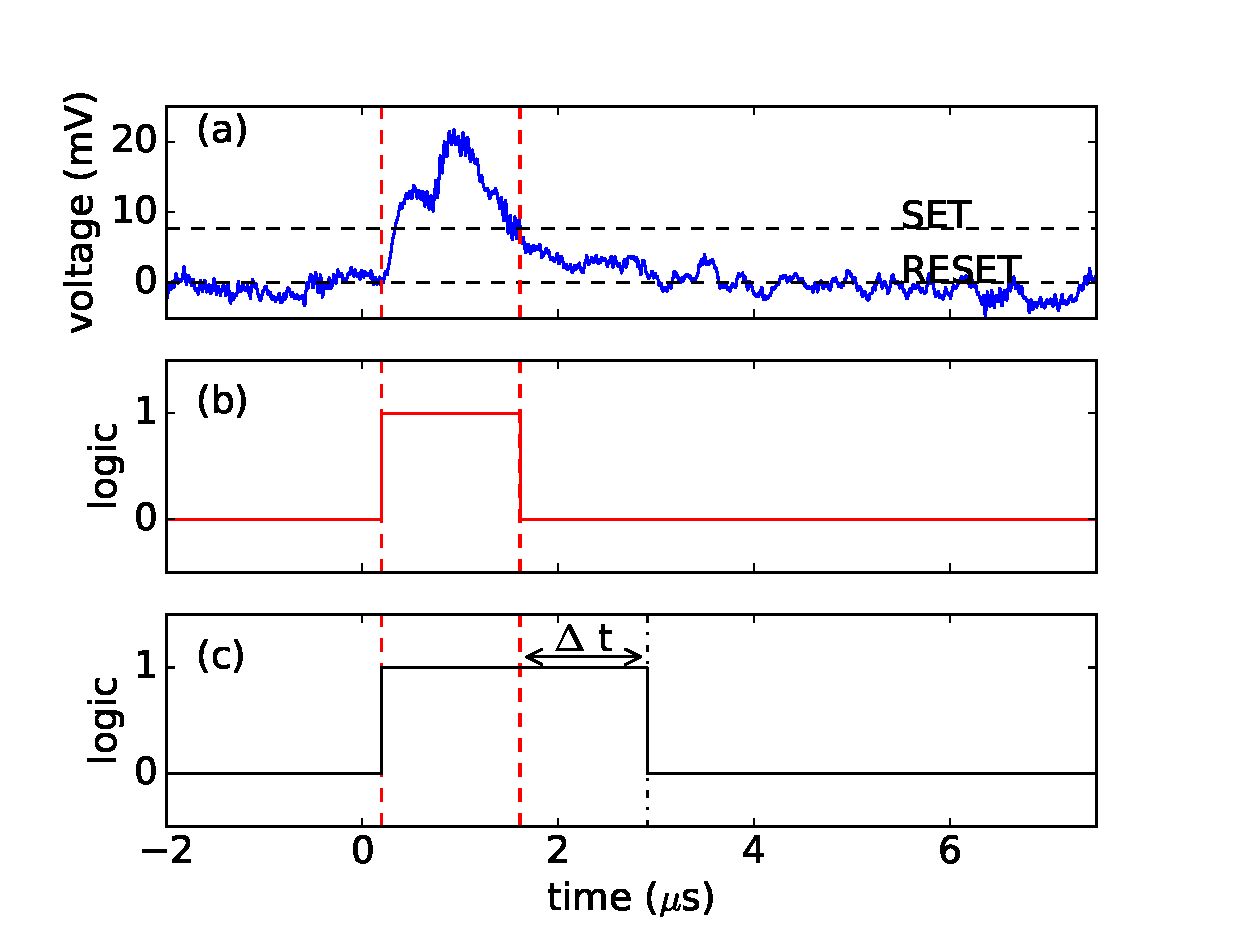
\includegraphics[width=1\linewidth]{figures/comparator/comparator_at_500ns.eps}
  \end{center}
  \vspace{-0.8cm}
  \figcaption{
	(a) Overlapping pulses separated by 482~ns. The rising edge of the later pulse is obscured by the earlier pulse and prevents arrival time estimation using the threshold crossing-time.
  (b) The two-level (discriminator) identifies the region corresponding to photon detection.
  (c) The discriminator logic extended by $\Delta t$ to include the decaying pulse tail. This mode is used to determine the pulse area.
}
\end{figurehere}
% \vspace{1cm}
% To determine the number of detected photons, we calculate the pulse area.
% To increase signal-to-noise ratio, we extend the discriminated region by $\Delta t=1300$~ns so that the decaying tail is included. 

\vspace{1cm}
\begin{center}
  \begin{center} {\bf \Large \textsf {Discriminator Initialisation}}\end{center}
\end{center}
To determine the SET voltage threshold $V_{th}$, 
we consider the maximum height distribution of the traces. 
%
We set $V_{th}$ to the value that minimizes the overlap between the height distributions corresponding to $n=0$ and $n>0$.

\begin{figurehere}
    \begin{center}
    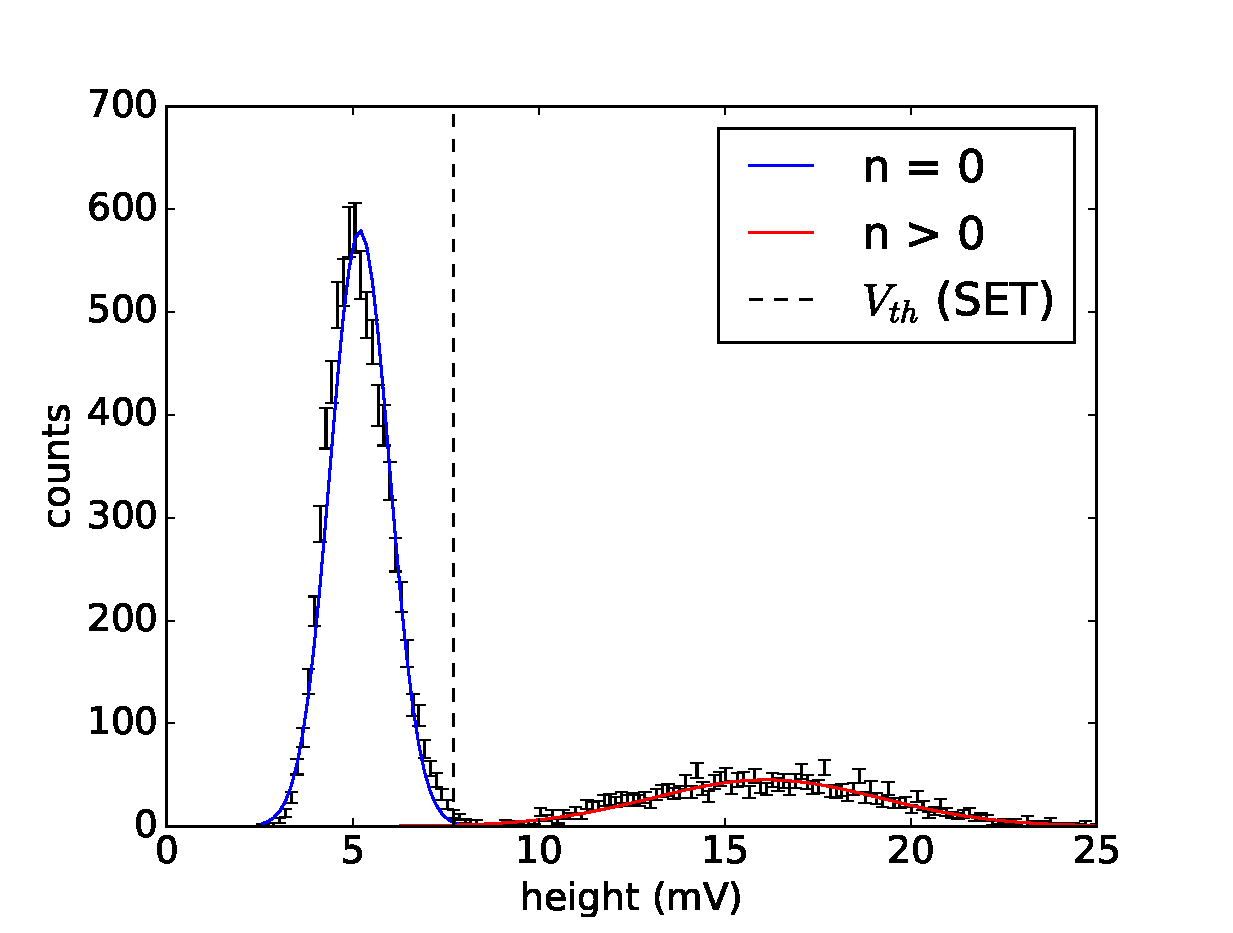
\includegraphics[width=0.9\linewidth]{figures/height_histogram_cw/height_histo.eps}
    \figcaption{\label{fig:height_histo}
        Pulse height histogram of the TES response to a CW LD emitting~$\bar{n} = 0.25$ photons in $10~\mu$s. The two peaks correspond to 0 and at least 1 photon being detected respectively. 
        Black line: Point of minimal overlap between Gaussian fits to the two height distributions corresponding to $V_{th} = 7.7$~mV.
        Error bars indicate Poissonian standard-deviation.
        }
    \end{center}
\end{figurehere}
